\documentclass{standalone}

\usepackage[OT1]{fontenc}
\renewcommand*\familydefault{\sfdefault}
\usepackage{helvet,sfmath}
\usepackage{siunitx}

\usepackage{tikz}
\usetikzlibrary{arrows,calc,patterns}
\usepackage{tikz,tkz-euclide}

\usetikzlibrary{decorations.markings}

%% midarrow
\tikzset{
    mid arrow/.style={
        decoration={markings, mark=at position 0.5 with {\arrow{stealth}}},
        postaction={decorate}
    }
}

%% Color
\definecolor{H_field}{RGB}{3, 49, 161}  % #0331A1
\definecolor{M_dipole}{RGB}{0, 127, 189} % #007FBD
\definecolor{J_Current}{RGB}{91, 199, 225} % #5BC7E1
\definecolor{Orange_note}{RGB}{248, 136, 16} % #F88810
\definecolor{P_dipole}{RGB}{201, 1, 161}  % #C901A1
\definecolor{E_field}{RGB}{113, 11, 121} % #710B79

\begin{document}

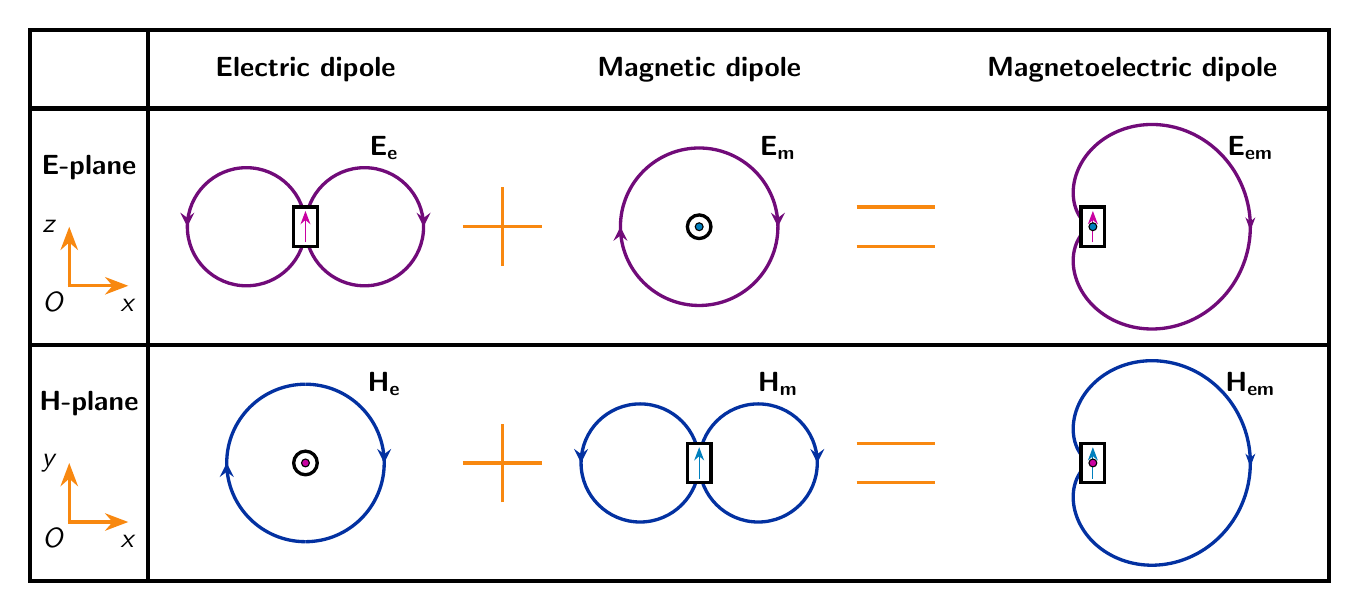
\begin{tikzpicture}[scale=0.5]
    %% Background
    \draw[ultra thick] (-17,-6) rectangle (16,0);
    \draw[ultra thick] (-17,0) rectangle (16,6);
    \draw[ultra thick] (-17,6) rectangle (16,8);
    \draw[ultra thick] (-17,-6) rectangle (-14,8);  

    \draw (-10,7) node{\textbf{Electric dipole}};
    \draw (0,7) node{\textbf{Magnetic dipole}};
    \draw (11,7) node{\textbf{Magnetoelectric dipole}};
    \draw (-15.5,4.5) node{\textbf{E-plane}};
    \draw (-15.5,-1.5) node{\textbf{H-plane}};

    %% Coordinate
    % xOz
    \draw[very thick, Orange_note, -Stealth] (-16.04,1.5) to (-14.5,1.5); 
    \draw[very thick, Orange_note, -Stealth] (-16,1.46) to (-16,3);
    \draw
    (-16.5,3) node{\(z\)}
    (-14.5,1) node{\(x\)}
    (-16.4,1.1) node{\(O\)}
    ;
    % xOy
    \draw[very thick, Orange_note, -Stealth] (-16.04,-4.5) to (-14.5,-4.5); 
    \draw[very thick, Orange_note, -Stealth] (-16,-4.54) to (-16,-3);
    \draw
    (-16.5,-3) node{\(y\)}
    (-14.5,-5) node{\(x\)}
    (-16.4,-4.9) node{\(O\)}
    ;
    %% Symbols
    \draw[very thick, Orange_note] 
    (-5,2) to (-5,4)
    (-6,3) to (-4,3)
    ;
    \draw[very thick, Orange_note] 
    (-5,-4) to (-5,-2)
    (-6,-3) to (-4,-3)
    ;
    \draw[very thick, Orange_note]
    (4,3.5) to (6,3.5)
    (4,2.5) to (6,2.5)
    ;
    \draw[very thick, Orange_note]
    (4,-3.5) to (6,-3.5)
    (4,-2.5) to (6,-2.5)
    ;
    
    %% Electric dipole yOz
    \draw[very thick, mid arrow, E_field] (-10,3) arc[start angle=0, end angle=360, radius=1.5];
    \draw[very thick, mid arrow, E_field] (-10,3) arc[start angle=180, end angle=-180, radius=1.5];
    \draw[very thick, fill = white] (-10.3,2.5) rectangle (-9.7,3.5);
    \draw[P_dipole, -Stealth] (-10,2.6) to (-10,3.4);
    \draw (-8,5) node{\(\mathbf{E_e}\)};

    %% Electric dipole xOy
    \draw[very thick, mid arrow, H_field] (-10,-1) arc[start angle=90, end angle=-90, radius=2];
    \draw[very thick, mid arrow, H_field] (-10,-5) arc[start angle=270, end angle=90, radius=2];
    \draw[very thick, fill = white] (-10,-3) circle (0.3);
    \draw[fill = P_dipole] (-10,-3) circle (0.1);
    \draw (-8,-1) node{\(\mathbf{H_e}\)};
    
    %% Magnetic dipole yOz
    \draw[very thick, mid arrow, E_field] (0,5) arc[start angle=90, end angle=-90, radius=2];
    \draw[very thick, mid arrow, E_field] (0,1) arc[start angle=270, end angle=90, radius=2];
    \draw[very thick, fill = white] (0,3) circle (0.3);
    \draw[fill = M_dipole] (0,3) circle (0.1);
    \draw (2,5) node{\(\mathbf{E_m}\)};

    %% Magnetic dipole yOz
    \draw[very thick, mid arrow, H_field] (0,-3) arc[start angle=0, end angle = 360, radius = 1.5];
    \draw[very thick, mid arrow, H_field] (0,-3) arc[start angle=180, end angle = -180, radius = 1.5];
    \draw[very thick, fill = white] (-0.3,-3.5) rectangle (0.3,-2.5);
    \draw[M_dipole, -Stealth] (0,-3.4) to (0,-2.6);
    \draw (2,-1) node{\(\mathbf{H_m}\)};
    
    %% Magnetoelectric dipole xOz
    \draw[very thick, color = E_field, domain=0:360, samples=100, smooth, variable = \t]
    plot ({10+2*(1+sin(\t))*sin(\t)}, {3+2*(1+sin(\t))*cos(\t)});
    \draw[very thick, fill = white] (9.7,2.5) rectangle (10.3,3.5);
    \draw[P_dipole, -Stealth] (10,2.6) to (10,3.4);
    \draw[fill = M_dipole] (10,3) circle (0.1);
    \draw[E_field, -Stealth] (14,3.1) to (14,2.9); 
    \draw (14,5) node{\(\mathbf{E_{em}}\)};

    %% Magnetoelectric dipole xOy
    \draw[very thick, color = H_field, domain=0:360, samples = 100, smooth, variable=\t] 
    plot ({10+2*(1+sin(\t))*sin(\t)}, {-3+2*(1+sin(\t))*cos(\t)});
    \draw[very thick, fill = white] (9.7,-3.5) rectangle (10.3,-2.5);
    \draw[M_dipole, -Stealth] (10,-3.4) to (10,-2.6);
    \draw[fill = P_dipole] (10,-3) circle (0.1);
    \draw[H_field, -Stealth] (14,-2.9) to (14,-3.1);
    \draw (14,-1) node{\(\mathbf{H_{em}}\)};
    
\end{tikzpicture}

\end{document}